\documentclass{article}

\usepackage{graphicx}
\usepackage{subfigure}
\usepackage[hypcap]{caption}
\usepackage{listings}
\usepackage{float}
\floatstyle{plaintop}
\restylefloat{table}

\title{Experimental Design and Data Analysis: Assignment 6}
\author{Andrew Bedard(2566978) \& Simone van Gompel(2567525) \\ Group 19}

\begin{document}

  \maketitle

  \section{Introduction}
    In this paper the process of analysing a certain dataset is laid out.
    The dataset used is calcium.dat, which can be found at \url{http://www.amstat.org/publications/jse/jse_data_archive.htm}.
    This dataset is used for this project is because it has a good number of entries and enough features to be able to do data analysis on.
    In the rest of this paper the experiment is explained, the data is analysed, the found results are shown and all of this will be discussed at the end.
    In the appendix the used R code is shown.

  \section{The Experiment}
    The experiment that was set up had as goal to see if age and sex has an influence on certain concentrations in the body.
    The concentrations that were measured are:
    \begin{itemize}
      \item Alkaline Phosphatase International Units/Liter
      \item Calcium mmol/L 
      \item Inorganic Phosphorus mmol/L
    \end{itemize}
    There are 6 different labs from which the data is extracted.
    Next to these features, the sex, age, agegroup and patient observation number are recorded.
    In the calcium.dat the original data is stored with errors, in calciumgood.dat the data is already cleaned up.
    In this project only the calcium.dat data is used to explain how the cleaning up of the data is done.

  \section{Data Analysis}
    First off a pairs plot was made of the data to be able to see how the data relates to each other.
    In Fig\ref{fig:FirstPairs} the foremost problem is clear, the outliers in the data are big and unlogical.
    Furthermore has Lab more than 6 categories, these problems can be explained by human error.
    And lastly the lab 3 has strange measurements with the cammol, this might be because of confusion of the measurement unit.
    The following values were changed:
    \begin{itemize}
      \item Removed Ages over 110
      \item Removed Sex which is not in the category 1 or 2
      \item Removed Lab categories which are over 6
      \item Removed Phosmmol over 2
      \item Divided Cammol of Lab 3 by 10 (this is visually tested by using a pairs plot)
    \end{itemize}
    After removal the same plot is made, see: Fig\ref{fig:SecondPairs}.
    Here you can see the correlations between the features better than in Fig\ref{fig:FirstPairs}.
    \begin{figure}[H]
        \centering
        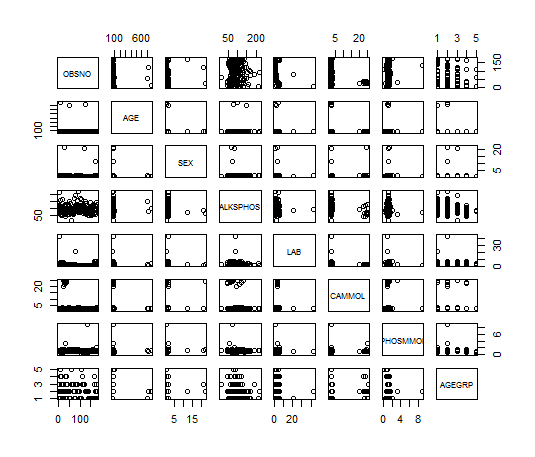
\includegraphics[scale=0.5]{../results/FirstPairs.png}
        \caption{Pairsplot of the original data}
        \label{fig:FirstPairs}
    \end{figure}
    \begin{figure}[H]
        \centering
        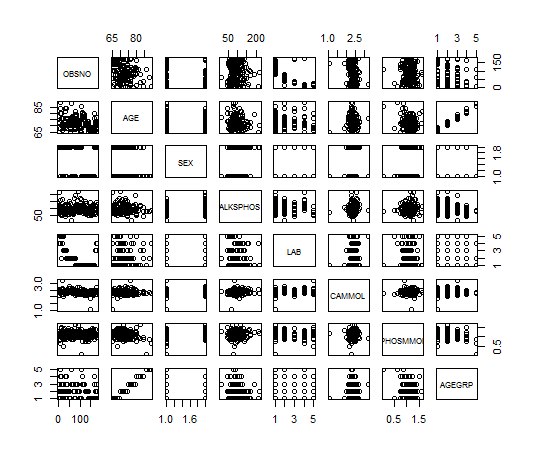
\includegraphics[scale=0.5]{../results/SecondPairs.png}
        \caption{Pairsplot of the updated data}
        \label{fig:SecondPairs}
    \end{figure}

  \section{Results}

  \section{Discussion}
    
  \section{R-Code}
    \begin{lstlisting}[language=R]
    \end{lstlisting}
\end{document}
